\chapter*{Konzeptentwurf}
\label{cha:Konzeptentwurf}

\section*{State Machine}
\label{sec:State Machine}

\subsection*{Initialzustand}
\label{subsec:Initialzustand}

Das System startet im Initialzustand und wechselt direkt in den sogenannten Idle-Zustand. Im Idle-Zustand sind beide LEDs der Anzeige AC2398 ausgeschaltet. In diesem Zustand kann das System je nach den erkannten Eingaben oder Ereignissen in andere Zustände wechseln. Wenn der grüne Knopf gedrückt wird und kein RFID-Tag erkannt wird, speichert das System die aktuelle Systemzeit und bleibt im Idle-Zustand. Dieser Vorgang wird im Diagramm als "Save Time" bezeichnet.

\subsection*{Tag-Erkennung und Verarbeitung}
\label{subsec:Tag-ErkennungundVerarbeitung}

Wird ein NFC-Tag erkannt und liegt kein Fehlerzustand vor, wechselt das System in den Zustand "Tag Detected Handling". In diesem Zustand blinkt die grüne LED mit einer Frequenz von einer Sekunde, um anzuzeigen, dass ein Tag erkannt wurde. Es gibt zwei mögliche Aktionen, vorausgesetzt, es liegt kein Fehlerzustand vor:

Write Tag Handling: Wenn der grüne Knopf gedrückt wird, während das RFID-Tag erkannt wird und die Systemzeit vorhanden ist, wechselt das System in den Zustand "Write Tag Handling". In diesem Zustand wird die zuvor gespeicherte Systemzeit auf das RFID-Tag geschrieben. Die grüne LED leuchtet dauerhaft, um anzuzeigen, dass der Schreibvorgang erfolgreich abgeschlossen wurde. Sobald das RFID-Tag nicht mehr erkannt wird, kehrt das System in den Idle-Zustand zurück.

Delete Tag Handling: Alternativ kann der rote Knopf gedrückt werden, während das RFID-Tag erkannt wird und kein Fehlerzustand vorliegt. In diesem Fall wechselt das System in den Zustand ''Delete Tag Handling''. Hier werden die gespeicherten Daten des RFID-Tags gelöscht, und beide LEDs leuchten dauerhaft, solange das Tag erkannt wird. Sobald das RFID-Tag nicht mehr erkannt wird, kehrt das System in den Idle-Zustand zurück.

\subsection*{Fehlerbehandlung}
\label{subsec:Fehlerbehandlung}

Wenn während des Prozesses ein Fehlerzustand auftritt, wechselt das System in den Zustand "Error State Handling". In diesem Zustand blinkt die rote LED mit einer Frequenz von einer Sekunde, während die grüne LED ausgeschaltet bleibt, um den Fehler anzuzeigen. Der Fehlerzustand bleibt bestehen, bis die Ursache des Fehlers behoben ist. Anschließend erreicht das System den Finalzustand und der gesamte Ablauf beginnt erneut.
\begin{figure}[h!]
	\centering
	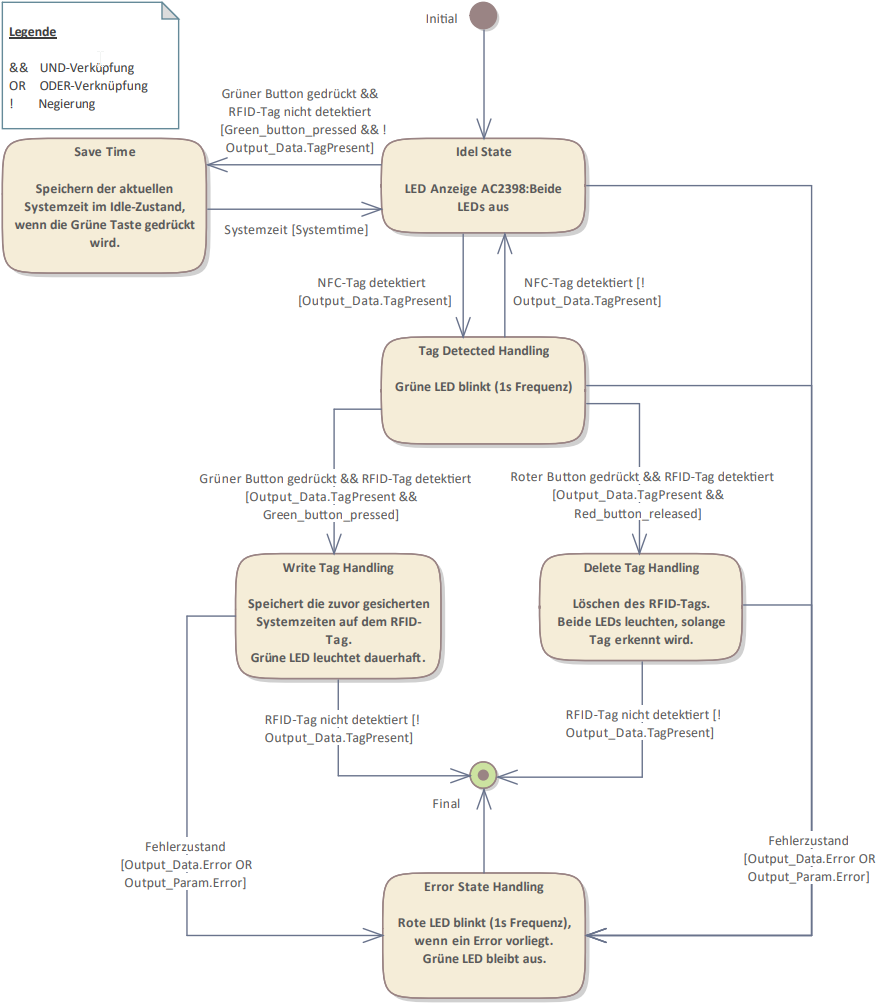
\includegraphics[width=1.0\textwidth]{images/StateMachine.png}
	\vspace{1cm}
	\caption{State-Machine-Diagramm}
	% [Abbildungsverzeichnis]{Bildunterschrift}
	\label{fig:StateMachineDiagramm}
\end{figure}

\clearpage
\newpage
\section*{Variablen-Tabellen}
\label{sec:VariablenTabellen}

Für die verwendete Hardware ''AC2398'' (ein Block mit zwei Tastern, jeweils mit integrierter LED) und das NFC-Modul ''DTI515'' werden die folgenden Variablentabellen (Tabelle \ref{tab:AC2398} und Tabelle \ref{tab:DTI515}) benötigt.

\begin{table}[h!]
	\centering
	\renewcommand{\arraystretch}{1.0} % Verringert den Zeilenabstand
	\footnotesize
	\begin{tabular}{|l|l|l|l|}
		\hline
		\textbf{Name} & \textbf{Datentyp} & \textbf{Adresse} & \textbf{Kommentar}\\ \hline
		RED\_button\_released & Bool & \%I193.2 & 1 wenn roter Taster nicht gedrückt \\ \hline
		Green\_button\_pressed & Bool & \%I193.3 & 1 wenn grüner Taster gedrückt \\ \hline
		Red\_button\_LED\_ON & Bool & \%Q192.0 & wenn 1 dann rote LED vom Taster an \\ \hline
		Green\_button\_LED\_ON & Bool & \%Q192.1 & wenn 1 grüne LED vom Taster an \\ \hline
	\end{tabular}
	\caption{Variablentabelle von AC2398 (Tasterblock)}
	\label{tab:AC2398}
\end{table}
\begin{table}[h!]
	\centering
	\renewcommand{\arraystretch}{1.0} % Verringert den Zeilenabstand
	\footnotesize
	\begin{tabular}{|p{6cm}|p{4.36cm}|p{3cm}|}
		\hline
		\textbf{Name} & \textbf{Datentyp} & \textbf{Adresse} \\ \hline
		Output\_Param.Done & Bool & \%I6.0 \\ \hline
		Output\_Param.Busy & Bool & \%I6.1 \\ \hline
		Output\_Param.Error & Bool & \%I6.2 \\ \hline
		Output\_Param.Status & Word & \%IW8 \\ \hline
		Output\_Param.ExtStatus & DWord & \%ID10 \\ \hline
		Output\_Param.RdValue & UInt & \%IW14 \\ \hline
		Output\_Data.TagPresent & Bool & \%I92.0 \\ \hline
		Output\_Data.Done & Bool & \%I92.1 \\ \hline
		Output\_Data.Busy & Bool & \%I92.2 \\ \hline
		Output\_Data.Error & Bool & \%I92.3 \\ \hline
		Output\_Data.Status & Word & \%IW94 \\ \hline
		Output\_Data.ExStatus & Word & \%IW96 \\ \hline
		Input\_Param.Execute & Bool & \%Q0.0 \\ \hline
		Input\_Param.Mode & UInt & \%QW2 \\ \hline
		Input\_Param.SetValue & UInt & \%QW4 \\ \hline
		Input\_Data.DT\_InAddr & UInt & \%QW16 \\ \hline
		Input\_Data.DT\_OutAddr & UInt & \%QW18 \\ \hline
		Input\_Data.Execute & Bool & \%Q20.0 \\ \hline
		Input\_Data.Force & Bool & \%Q20.1 \\ \hline
		Input\_Data.Mode & UInt & \%QW22 \\ \hline
		Input\_Data.TagMemAddr & UInt & \%QW24 \\ \hline
		Input\_Data.Length & UInt & \%QW26 \\ \hline
		Input\_Data.WrData & Array[0..31] of Byte & \%Q28.0 \\ \hline
		Input\_Data.RdData & Array[0..31] of Byte & \%Q60.0 \\ \hline
	\end{tabular}
	\caption{Variablentabelle von DTI515 (NFC-Modul)}
	\label{tab:DTI515}
\end{table}

Zur Realisierung der in Abbildung \ref{fig:StateMachineDiagramm} dargestellten Logik werden die bausteinlokalen Variablen aus Tabelle \ref{tab:BausteinlokaleVariablen} benötigt. Diese Variablen werden später im Funktionsbaustein ''FB\_RFID\_Manager'' deklariert.

\begin{table}[h!]
	\centering
	\renewcommand{\arraystretch}{1.0} % Verringert den Zeilenabstand
	\footnotesize
	\begin{tabular}{|l|p{1.7cm}|p{5.6cm}|} % p{10cm} sorgt dafür, dass die Kommentare umbrochen werden
		\hline
		\textbf{Name} & \textbf{Datentyp}  & \textbf{Kommentar} \\ \hline
		Tag\_Present & Bool & Wird ein NFC\_Tag erkannt \\ \hline
		Clock1Hz & Bool & Eine Clock mit 1 Herz \\ \hline
		Green\_button & Bool & Wird Grüner Button betätigt \\ \hline
		Red\_button & Bool & Wird Roter Button losgelassen \\ \hline
		Data\_Error & Bool & Fehler im Read/Write Data FBD \\ \hline
		Paramter\_Error & Bool & Fehler im parametrization FBD \\ \hline
		Execute & Bool & Ausführung des Schreibe bzw. Lösch Vorgangs \\ \hline
		Green\_Button\_LED\_State & Bool & Status der LED des grünen Buttons \\ \hline
		Red\_Button\_LED\_State & Bool & Status der LED des roten Buttons \\ \hline
		Data\_Mode & Int & Welcher Modus verwendet wird \\ \hline
		Data\_Write & Array[0..31] of Byte & Eine Liste zum speichern der geschriebenen bzw. gelöschten Bytes \\ \hline
		Data\_Length & Int & Einstellung der Länge der Liste am FBD Read/Write Data \\ \hline
		M1\_Error\_State\_Handling & Bool & Netzwerk 1: Wird ein Fehler erkannt? \\ \hline
		M2\_Error\_State\_Handling\_Clock & Bool & Netzwerk 2: Clock aktiv? \\ \hline
		M3\_Tag\_Detected\_Handling & Bool & Netzwerk 2: Wird ein NFC-Tag erkannt? \\ \hline
		M4\_Tag\_Detected\_Handling\_Clock & Bool & Netzwerk 2: Clock aktiv? \\ \hline
		M5\_Save\_System\_Time & Bool & Netzwerk 3: Wurde einmal die Zeit gespeichert? \\ \hline
		M6\_Write\_Tag\_Handling & Bool & Netzwerk 4: Wird auf den NFC-Tag geschrieben? \\ \hline
		M7\_Delete\_Tag\_Handling & Bool & Netzwerk 5: Wird der NFC-Tag gelöscht \\ \hline
		Green\_LED\_Tag\_Detected\_Handling & Bool & Grüne LED wird eingeschaltet, wenn Tag erkannt wird \\ \hline
		Green\_LED\_Write\_Tag\_Handling & Bool & Grüne LED wird eingeschaltet, wenn NFC-Tag beschrieben wurde \\ \hline
		Green\_LED\_Delete\_Tag\_Handling & Bool & Grüne LED wird eingeschaltet, wenn NFC-Tag gelöscht wurde \\ \hline
		Red\_LED\_Error\_State & Bool & Rote LED wird eingeschaltet, wenn ein Fehlerzustand herrscht \\ \hline
		Systemtime & Bool & Speicher Systemzeit im Format Time \\ \hline
		Systemtimeconv & Bool & Gespeicherte Systemzeit wird Datentyp DInt konvertiert \\ \hline
		Execute\_Write\_Handling & Bool & Ausführung des Schreibbefehls \\ \hline
		Execute\_Delete\_Handling & Bool & Ausführung des Löschbefehls \\ \hline
	\end{tabular}
	\caption{Bausteinlokale Variablen von Funktionsbaustein ''FB\_RFID\_Manager''}
	\label{tab:BausteinlokaleVariablen}
\end{table}

% ------------------------------------------------------------------------------------
%... Text Konzeptentwurf: Gegenüberstellung verschiedener Lösungsansätze und Lösungsgenerierung, etc.